\documentclass{article}
\usepackage[utf8]{inputenc}
\usepackage{graphicx}
%\usepackage[section]{placeins}

\title{Assignment 8 Report}
\author{Bharat Jindal}

\begin{document}
\maketitle

\section{Plot 1}
Plot 1 provides graphs of 100 iterations for some Number of Elements against Execution time while varying Number of Threads running in parallel.
\begin{figure}[htb!]
\centering
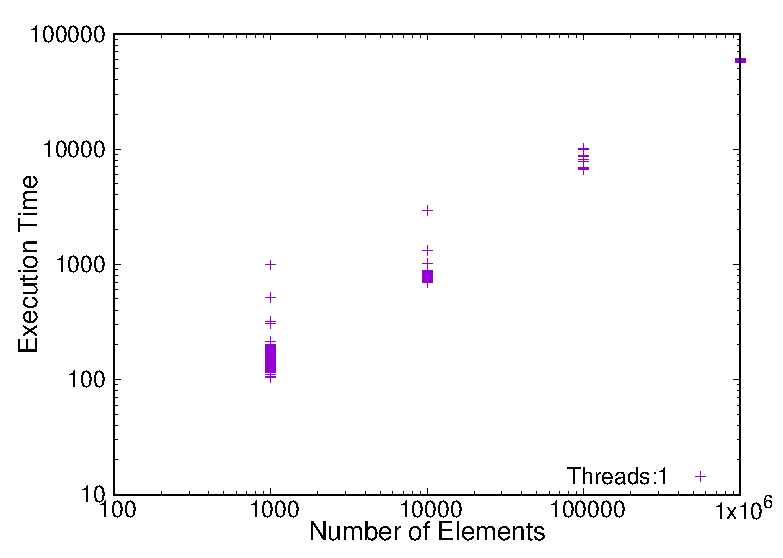
\includegraphics[scale=0.9]{plot1_1.eps}
\caption{Plot 1 Threads = 1}
\end{figure}

\begin{figure}
\centering
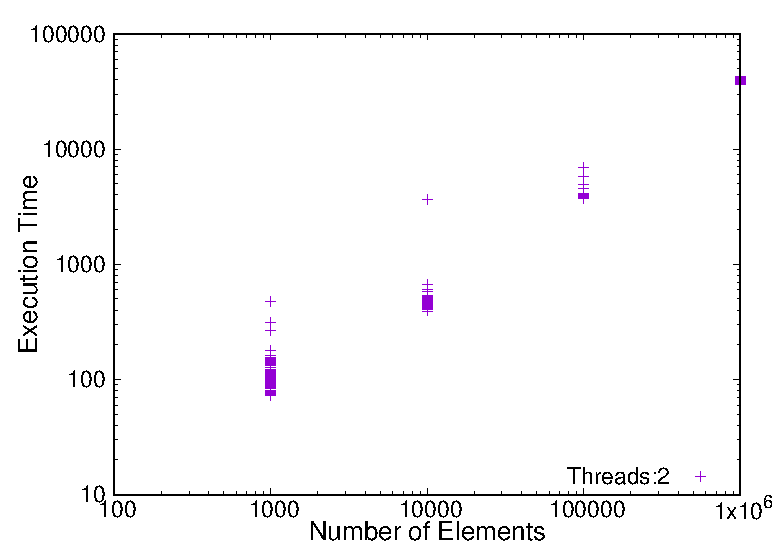
\includegraphics[scale=0.9]{plot1_2.eps}
\caption{Plot 1 Threads = 2}
\end{figure}

\begin{figure}
\centering
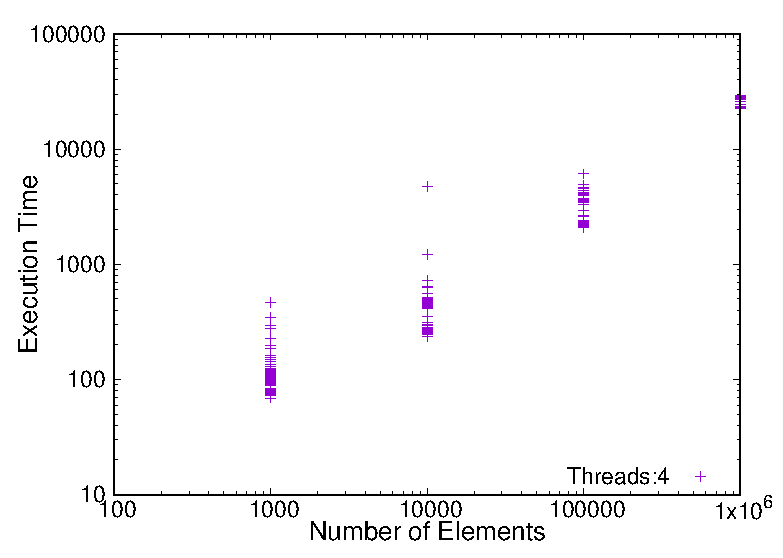
\includegraphics[scale=0.9]{plot1_4.eps}
\caption{Plot 1 Threads = 4}
\end{figure}

\begin{figure}
\centering
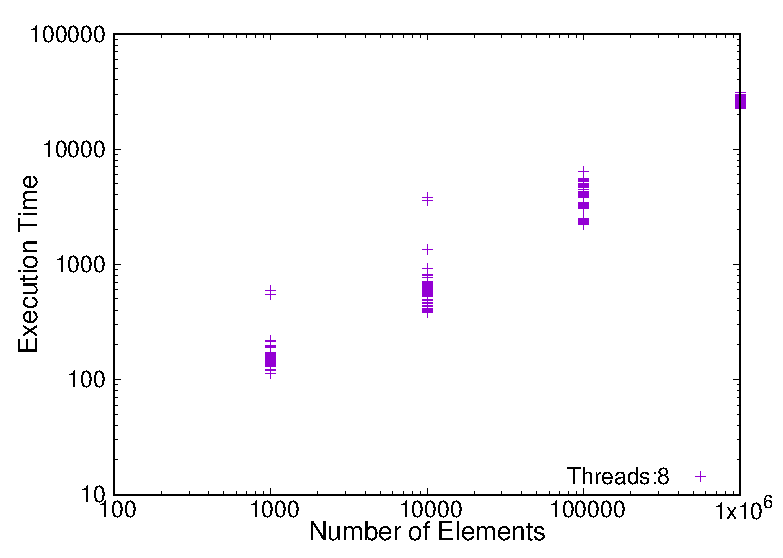
\includegraphics[scale=0.9]{plot1_8.eps}
\caption{Plot 1 Threads = 8}
\end{figure}

\begin{figure}
\centering
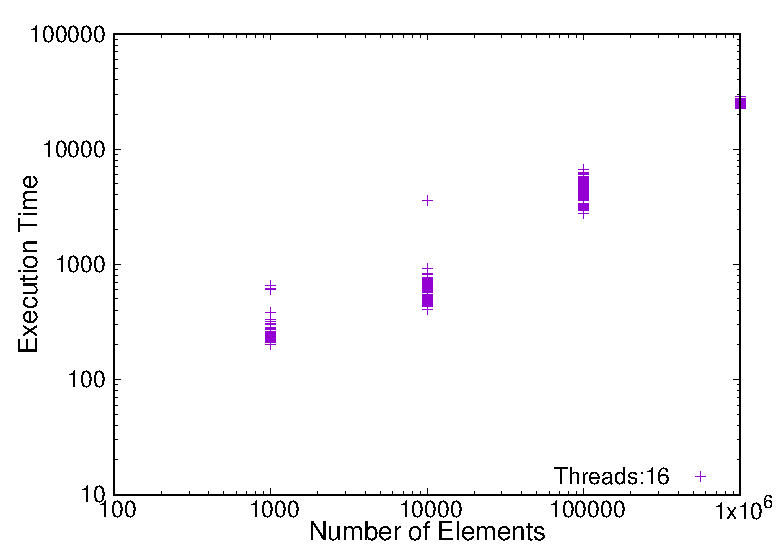
\includegraphics[scale=0.9]{plot1_16.eps}
\caption{Plot 1 Threads = 16}
\end{figure}

\section{Plot 2}
Plot 2 depicts the average of 100 iteration's execution time for various threads in linepolot.
\begin{figure}[htb!]
\centering
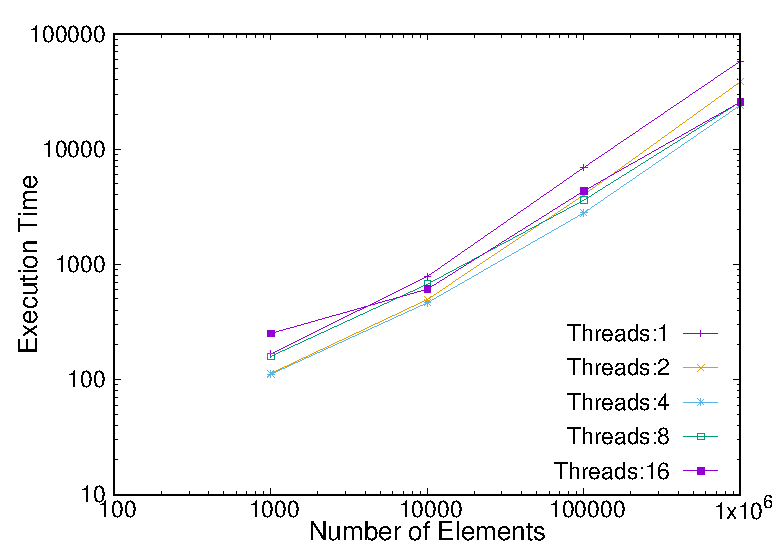
\includegraphics[scale=0.9]{plot2.eps}
\caption{Plot 2}
\end{figure}

\section{Plot 3}
Plot 3 is depicting as histograms effect of changing number of threads for particular number of inputs.
\begin{figure}[htb!]
\centering
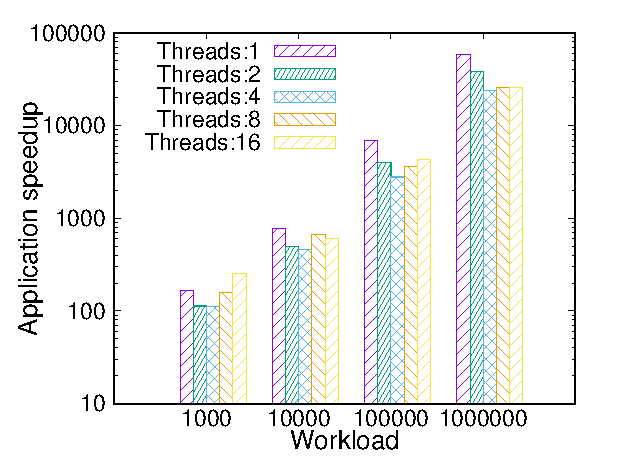
\includegraphics[scale=0.9]{plot3.eps}
\caption{Plot 3}
\end{figure}

\section{Plot 4}
Additional information then that of plot 3 is that it is also showing Standard Deviation of execution time.
\begin{figure}[htb!]
\centering
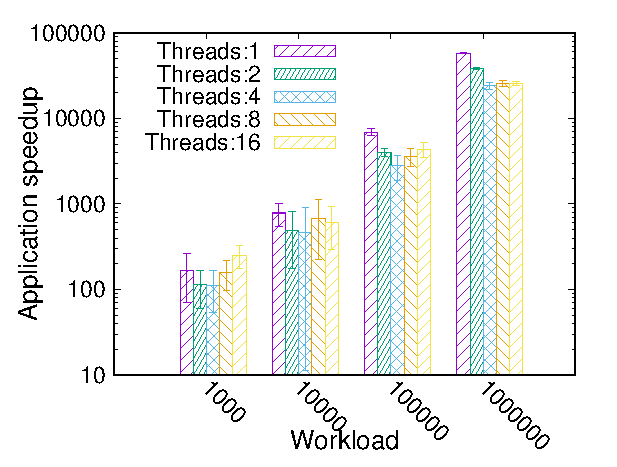
\includegraphics[scale=0.9]{plot4.eps}
\caption{Plot 4}
\end{figure}


\end{document}
